\section{Experiment Implementation}
\label{sec:implementation}
\noteby{KL}{This section will be deleted. Leaving it in for now so Vector can cut and paste from it.}

Section~\ref{sec:methodology} introduced the methodology at a conceptual level.
However, as with any real world measurement, we need to account for different
possible scenarios, and also take into consideration what works best with the
{\reflectors}. In this section, we first explain the implementation detail of
our {\reflector} selection, then we discuss the design of the blocking detection
experiment and false positive and false negative evaluation. Finally, we look
at how to exactly sample IPs from blacklists.

%\subsection{Measurement Infrastructure}
%Even at the conceptual level, it is evident that the measurement hinges
%on our ability to do two things. One, spoof IP addresses. Second, the
%ability to send many ``probe'' packets to hosts without getting blocked.
%For the first we got two machines that allowed us to spoof IPs outside
%our organization's source address validation zone. For the second part,
%we leveraged unused address space in the address space controlled by our
%organization. We configured multiple /24s to effectively point to a single
%machine so that we could cycle through many IPs from different /24s so that
%we do not burn our IPs.
%\textcolor{red}{maybe change organization to university?}
%\textcolor{red}{maybe have a small figure?}

\subsection{{\reflectorcap} Selection}

We use the daily scanning data from Censys~\cite{censys} as the starting point.
Censys scans the Internet daily and maintains a list of the daily active hosts
and their open ports. We took a snapshot of the Censys data on
\textbf{November 8th 2019} and then filtered them so that we are only left
with US hosts, which leads to about 40 Million hosts. We then scan these hosts
and identify suitable candidates -- hosts which have a shared global
monotonically increasing IP ID counter. We achieve this by sending multiple
probes to each host targeting an open port from different source addresses
and observing the responses. In the case where hosts have multiple open
ports, we randomly select a port to send the probe.

To identify stateful firewall, we send SYN-ACK packets to each host in two
different pattern: 1 second per packet with 24 packets, and 5 packets per second
with 60 packets, which correspond to the speed we probe {\reflectors} during
actually experiments(see the following section). We repeat each experiment 6
times and discard the hosts that blocked us after the experiment. To filter out
the hosts with low extra traffic, we send 24 probe to each host, 1 per second,
and repeat the experiment 5 times(in different time of the day). We then
collect the result and only select the hosts where more than 30\% of their IP
ID increases are equal to 1 per second (meaning in that second, the host did not
receive any extra traffic besides our probes), and all of these changes are
smaller than 10 within each second.

Finally, we try to identify the hosts with ingress filtering. In order to account
for differences in ingress filtering that may possibly occur on different path
to the {\reflectors} we acquired 7 vantage points in order to exercise
different paths. We then send spoofed packets from our measurement
machine to the {\reflectors} with spoofed source IP address corresponding to
the 7 vantage points, and we finally collect responses at each of the 7
vantage points. We only select the {\reflectors} that send responses to all 7
vantage points, meaning they did not drop any of our spoofed packets.

Eventually, we identified {\reflcount} IP addresses in US \footnote{We initially
discovered more than 300K {\reflectors}, but during our experiments, some hosts
became inactive. The number reported here are the final number after we finished
all our experiments.} that meet our requirements.
For the purpose of this paper, here we treat each individual IP
address as a distinct {\reflector}. Detail numbers are presented in
Table~\ref{tab:target-hosts}.

\begin{table}
\centering
\caption{The number of {\reflectors}(IP addresses) identified in United States, and the
corresponding count of /24, Autonomous systems and organizations (One
organization can have multiple ASes)}
\label{tab:target-hosts}
\footnotesize
\begin{tabular}{l >{\hfill}p{4.5cm}}
 \toprule
 Category                    &  Count    \\
 \midrule
 \textbf{IP Addresses}       &  \reflcount  \\
 \textbf{/24 Count}          &  128,712  \\
 \textbf{Autonomous Systems} &  3,371    \\
 \textbf{Organizations}      &  3,321    \\
 \bottomrule
\end{tabular}
\end{table}



\subsection{Experiment Design}

Previously, we described the theoretical model of our measurement method,
which explained the idea and workflow at a high-level. However, this model
does not take into consideration packet loss and extra traffic at
$Host_A$. As one would expect this is an unrealistic assumption in a real
world scenario, as packet loss can happen at many stages during the transit.
Furthermore, there is no guarantee that the host with an open port online
will not get any other traffic. Thus, to perform the measurement in real
world, we need to take all these factors into consideration and make sure
that our analysis model is robust to these real world uncertainties.

Besides that, our detection methodology also needs to be \textit{efficient},
\textit{accurate}, and have a \textit{low overhead}. Since we need to
measurement every pair of \texttt{<{\reflector}, blacklist IP>}, which is a
massive number, and also blacklist content is changing rapidly,
the detection method needs to be efficient so that we can finish the
measurement in a reasonable amount of time. The method should also have a low
false positive and false negative rate, so we can be confident about the result.
Finally, it should requires as less packets being sent as possible, both to
meet network bandwidth limitation on our measurement machine side, and to
generate less noise to the {\reflectors}.

We define a \textit{trial} as a single
measurement that tests if a {\reflector} blocks a blacklist IP.
Figure~\ref{fig:design_implementation} shows the process of one trial in
detail. For each trial, the measurement machine sends 5 consecutive
\textit{probe packets} to the {\reflector}, with each packet being sent 1
second apart. In our experiment, the probe packets are TCP SYN-ACK packets
and we get IP IDs from responded RST packets. Between the 3rd and 4th probe
packets, the measurement machine sends 5 \textit{spoofed packets}, also TCP
SYN-ACK, with source IPs equal to the blacklist IP. And between the 4th and
the 5th probe packets, it sends another 5 spoofed packets. Each time we send
the 5 spoofed packets, we send them 0.15 second apart consecutively, making
them spread across the 1 second window between two IP ID probes.

\begin{figure}[t]
\centering
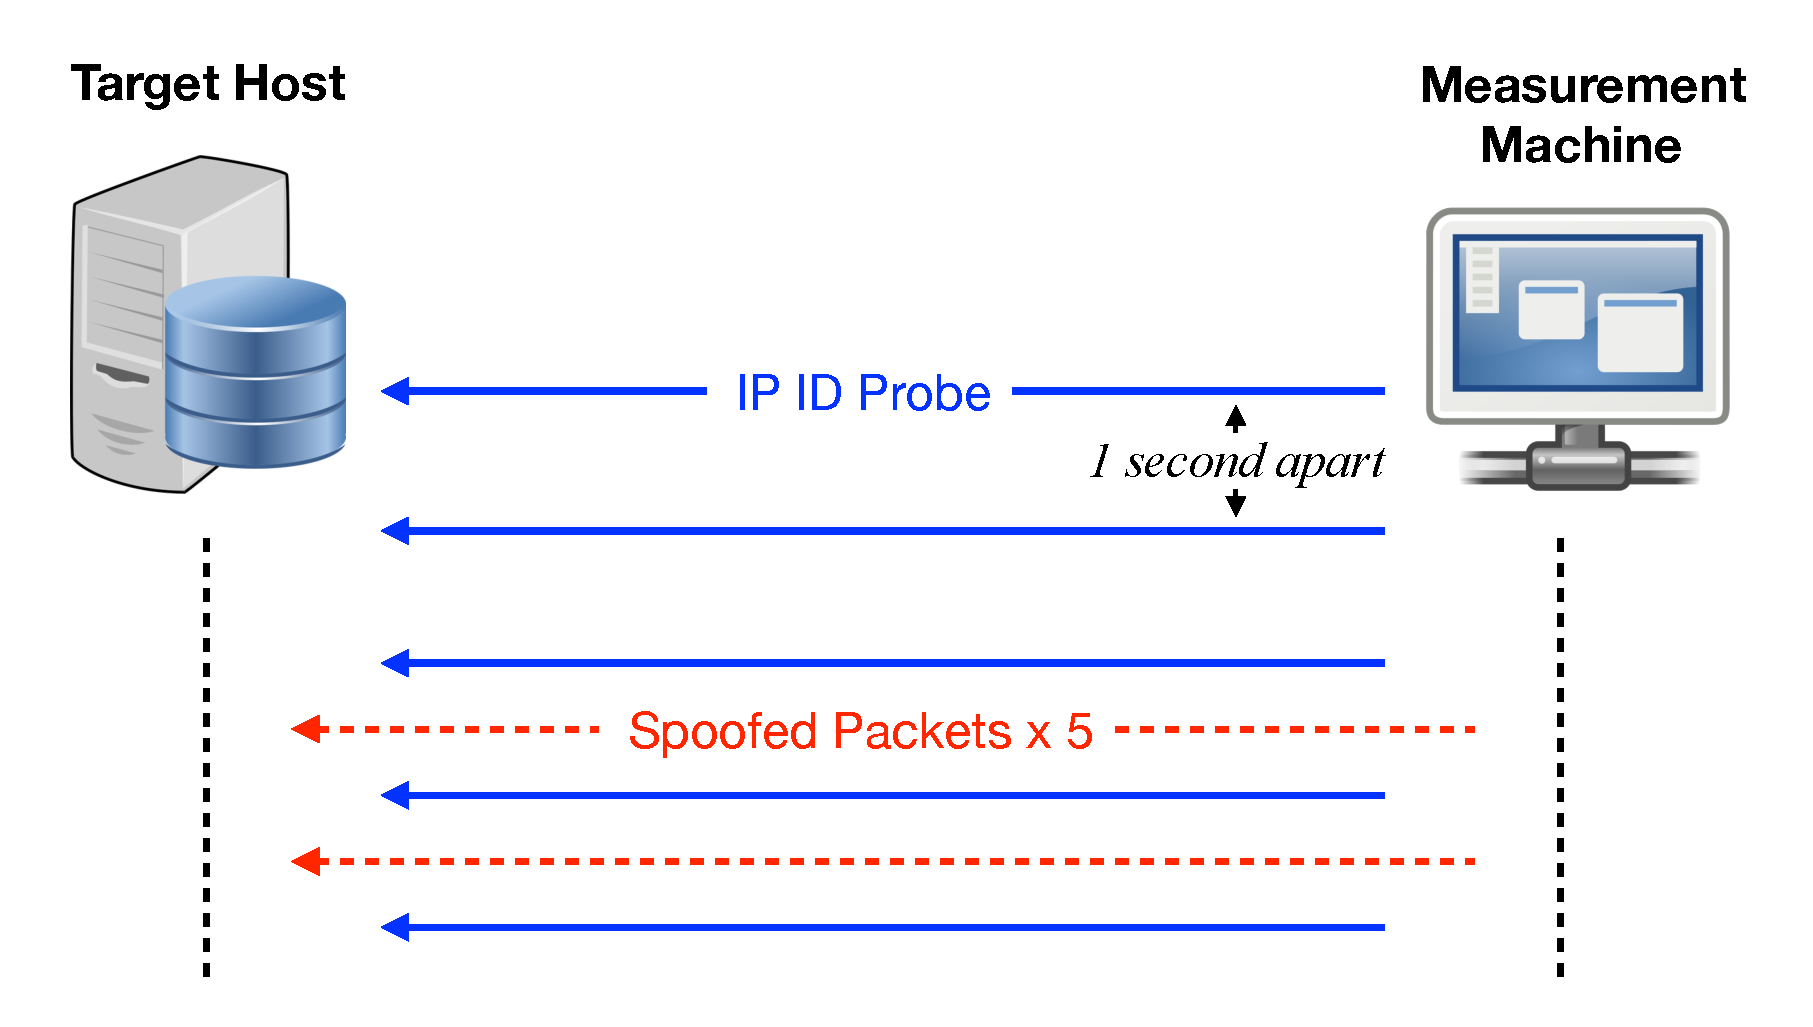
\includegraphics[width=0.85\columnwidth]{images/croped_design_implementation.pdf}
\caption{Blocking detection method used in this paper. The solid blue line present
the \textit{probe packets}, where we get the IP ID from the response, and dashed red line
present \textit{spoofed packets}, where we spoof packets impersonate IP from
blacklists, and trigger the extra changes of the {\reflectors}' IP ID.}
\label{fig:design_implementation}
\end{figure}

Now, we look at the deltas between the IP IDs for the packets received by the
measurement machine. In an ideal world, when there is no other traffic
generated by the {\reflector}, and no packet loss during our measurement, we
should observe that the IP ID increase between consecutive probes by exactly
1, and for the last two delta, since we send the spoofed packets in between
our probe packets, the final IP ID increases will be different based on the
host's blocking behavior.

If the host does not block the blacklist IP, then
we will observe an IP ID increase sequence in our received RST responses as:
\[[\hspace{0.1cm} +1, +1, +6, +6 \hspace{0.1cm}]\]
Here the last two deltas are +6 since the {\reflector} does not block the
blacklist IP and thus responds to spoofed packets, causing IP ID to increase by
5, and our probe packet causes it to increase by another 1, which gets us to +6.

On the other hand, if the host blocks the blacklist IP, then we will see an IP
ID increase sequence as:
\[ [\hspace{0.1cm} +1, +1, +1, +1 \hspace{0.1cm}] \]
Here the last two deltas are +1 since the {\reflector} blocks the blacklist IP,
leading to no extra change in IP ID.
%\textcolor{red}{maybe have an example of what happens when we do not see ideal conditions}

The first three probes -- corresponding to the first two IP ID deltas -- act as a
control. The last two ``probe and spoof'' patterns serve the actual measurement.
Seeing the initial two ``+1'' indicates this host is in a quiet period --- no
extra network traffic. Therefore, we can be more confident that the following
IP ID accelerate(``+6'' in our case) is because of our experiment. However,
while we present the choice of the numbers in the experiment as fait accompli,
there is a rationale behind the choice of numbers which we discuss later in
this section.

\textbf{Inference Criteria: }
Now we discuss how to infer whether a {\reflector} is blocking a blacklist IP
in real world. We have limited vantage point from the measurement machine, as
such, we have no knowledge of what happened on the {\reflector}, and our
information is limited to the IP IDs we see from the {\reflector}. Therefore,
we would like to be very conservative when making a judgment. In this
measurement, our approach is to try the same trial, between a {\reflector} and a
blacklist IP, many times until we get a ``perfect signal'' --- a response
which matches all the criteria below:

\begin{enumerate}
    \item The measurement machine received exact 5 RST responses from the {\reflector}.
    \item The 5 responses are received 1 second apart consecutively.
    \item The IP ID delta sequence in the 5 responses are either [+1, +1, +6, +6],
    which we will conclude as no blocking, or [+1, +1, +1, +1], which we will
    conclude as blocking.
    \item If any of the above 3 criteria is not met, we repeat the same experiment again.
    We repeat up to 15 times before giving up.
\end{enumerate}

Essentially, the first requirement ensures no packet loss. The second
requirement ensures responses we received reflect the real IP ID changes in
the {\reflector}. Internet does not guarantee the order of packet arrival.
Although we send one probe packet per second, and then send the spoofed
packets in between of the probe packets, these packets might not arrive at
the {\reflector} in the same order. Similarly, the response packets might be
reordered. Therefore, the IP ID sequence we get from the responded packets
might not represent the real order of IP ID changes in the host. Enforcing
the received response packets are also close to 1 second apart, we minimize
the probability of the reordered packets. In our experiment, we enforce that
the response packets can not be less than 0.85 or more than 1.15 second
apart.

The third requirement is the core of our inference logic. We want to be
conservative when concluding whether there is blocking or not, so we will
make the judgment only when we observe an IP ID delta sequence [+1, +1, +1,
+1] or [+1, +1, +6, +6], and ignore everything else. Then if we saw a
sequence of [+1, +1, +1, +1] but the host is not blocking the blacklist IP,
that would mean all the 10 spoofed packets were lost during the transmit. On
the other hand, if we see [+1, +1, +6, +6] and the host is actually blocking
the blacklist IP, then that would mean during our experiment, there are
exactly 5 extra packets generated by the host during each of the last two
window. Both cases are very unlikely to happen, and we will show a concrete
analysis of false positives and false negatives in the remainder of this section.


\textbf{False Positive and False Negative Analysis: }
For our experiment, we define ``false positive'' to be when a host is not
blocking a blacklist IP, but we mistakenly conclude it is blocking. On the
other hand, we define ``false negative'' to be when a host is blocking a
blacklist IP, but we mistakenly conclude it is not blocking. With
{\reflectors} being collected, we can actually empirically evaluate the
probability of a false positive or a false negative.

For false positive evaluation, we first acquire a list of IPs that are verified
not being blocked by {\reflectors}. Since we own these IPs, we can easily verify
that by directly probing the hosts from these IPs. We have acquired and tested
1,265 IPs from 5 different /24s. Then we probe {\reflectors} and send the
spoofed packets with source addresses being these pre-selected IPs. Since we
know that these IPs are not blocked, if we observed an IP ID delta sequence
[+1, +1, +1, +1], then it is a false positive case. For false negative, we run
the experiment with only probe packets, and no spoofed packets. This is
equivalent to the scenario when the host blocked the spoofed packets. Then if
we observed a delta sequence [+1, +1, +6, +6], then we know it was due to the
background traffic at the {\reflector} and hence is a false negative.

So far we have not explained our experiment design choice of spoofing 5 packets
per second. In fact, we tested with a range of numbers and calculated
their false positive and negative rates. We tested with spoofed packets equal
to 3, 4, 5, 6, 7 respectively. For each number, we use 15 distinct IPs we own
as the source addresses to spoof, and there is another group where we do not
spoof any packets. We repeat each test 4 times and do the overall experiment
twice. The final results are shown in Figure~\ref{fig:fp_fn_analysis}.

%Our goal is to minimize the false positives and false negatives while also keeping
%in mind the amount of traffic we generate. Additionally, we have a few dimensions
%of the experiment which we can adjust to reach this goal. Namely, the number of
%packets we spoof, and the number of times we spoof.
%To find these optimal numbers, we test with a range of numbers and calculate

\begin{figure}[t]
\centering
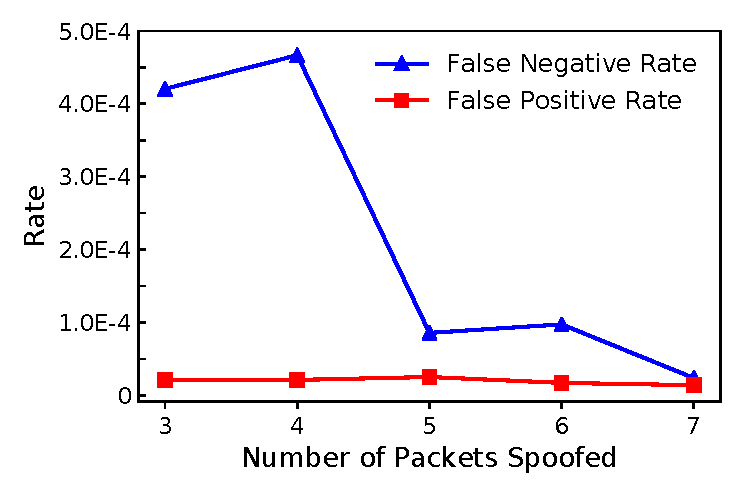
\includegraphics[width=0.85\columnwidth]{images/false_positive_negative.pdf}
\caption{False positive rate and false negative rate of the technique when
spoofing different amount of packets}
\label{fig:fp_fn_analysis}
\end{figure}

A few things stand out. The false negative rate drops significantly when we
send 5 spoofed packets. Surprisingly, the false negative rate jumps up
slightly when we spoof 6 packets. On the other hand, the false positive rate
keeps marginally trending downwards as we increase the number of spoofed
packets. We try to make the trade-off between having low false positive and
negative rates, but at the same time generating as less traffic as possible.
We choose 5 spoofed packets as a balance. By sending 5 spoofed packets, we
get a false positive rate of 2.5e-5, and a false negative rate of 8.5e-5.

Furthermore, we also tested strategies where we send 4 probe packets, from which
we get 3 IP ID deltas, and send 6 probe packets, from which we get 5 IP ID
deltas. With only 3 deltas we suffer a higher false negative rate, as it is
easier for the {\reflector} to show the same IP ID increase sequence with
extra traffic. With 6 probes, on the other hand, we prolong the experiment,
and more importantly, it is harder for us to get the ``perfect signal'' since
it is harder to capture a period with no other traffic when the time window
is longer. Thus, our choice of 5 probe packets with 5 spoofed packets in
between is essentially a trade off.

%We choose to send 5 probe packets because it is a balance between getting
%enough sample point of IP ID to see the changes, and not sending too many
%packets to the {\reflector} that might affect the host, as we need to repeat
%the experiment many times for many different blacklist IPs. The first three
%probes (where we get the first two IP ID delta) act as a control, and the
%last two probe and the spoof packets serve the actually experiment. The
%choice of 5 spoofed packets between each second is also the result of
%balance. If we send too little spoofed packets, then it is hard to argue
%whether the additional IP ID increments come from our spoofed packets or the
%hosts' own third-party traffic. If we send too many spoofed packets, it is
%hard to ensure they will arrive the host exactly between the probe packets,
%and also might trigger some stateful firewall logic, as we discussed in
%Section~\ref{sec:requirement}.


\subsection{Blacklist IP Sampling}
%How we selected the target blacklists
Given a blacklist feed to test, we need to ensure the sampled IPs meet the
requirements stated in Section~\ref{sec:requirement_list}. In order to
satisfy those requirements we need to utilize external data.

The ``exclusive'' requirement indicates that the IPs we used should be unique
to that blacklist -- that is no other blacklist that we have access to should
have them. In this paper, we utilize the FireHOL IP blacklist
collection~\cite{firehol}, a public service that collect data from over 100
public popular IP blacklists everyday. We use the public IP blacklists
collected by FireHOL to calculate the exclusive part of each target blacklist.

For the ``stable'' requirement, we collect all the target blacklists hourly,
and ensure the sampled IPs are in the blacklist throughout the corresponding
experiments.

To meet the ``routable'' requirement, we use the daily RouteView
Project~\cite{Routeview} data to identify BGP routable IPs, and further check
their whois record to confirm. For geo-location information, we use
Netacuity~\cite{netacuity} to identify each IP's location, and make sure for
each experiment, the sampled IPs cover as many different countries as the
data allows.

%\subsection{Representative}

%\subsubsection{Are reflectors representative}
%One concern is that our reflector selection biases our measurement to only
%include hosts that are low traffic. A second concern is if the networks are
%themselves representative?

%we are conservative in our reflector selection. One can imagine we relax our
%constraints and use a statistical approach to classify reflectors (as seen in
%Augur paper).

%Stats on reflector distribution.
%\subsubsection{Are blacklists representative}
